





%\section{Methods}\label{sec:Methods}

\subsection{Map imagery sampling.}\label{sec:methods2}
The concept employed in this study was to sample maps of individual city sections, calculate block size and regularity of each section, and then use a self organising map (SOM) to organise the images into different urban types. All cities with populations greater than 300,000 people\cite{UN2014} were selected for analysis. Map imagery from Google Maps\cite{GoogleStatic2017} was used to provide globally consistent data. 

A two-stage sampling approach was applied to each city. As no standardised urban boundaries are available for all the cities evaluated in this study, a methodology had to be developed to define these. Firstly, a sampling area extending 1.5 km from the identified city centroid\cite{UN2014} was set as a baseline. Then the sampling radius $r$ (km) was scaled, increasing by a power of 0.85 to the proportional increase in population size based on Barthelemy\cite{Barthelemy2016} in 

\begin{equation}
r = \sqrt{ \frac{28.27}{\pi} \left( \frac{p}{300,000} \right) ^{0.85} }
\end{equation}


Standardising the sampling area in this manner avoided socio-political discrepancies relating to a city's `true' (political) boundary and captured differences in population density and shape between small (e.g., Wellington, New Zealand; Izmit, Turkey) and global mega-cities (e.g., Tokyo, Japan; Delhi, India). Location sampling areas were adjusted for the earth's curvature\cite{Sinnott1984}. Large water-bodies (e.g., oceans but not coastlines) were removed from the sampling area, as they were not indicative of urban form. 

These procedures result in a population and water body-adjusted circular area centred on the city's central coordinates, intended to capture the widest extent of each city while minimising the amount of non-urban locations. For example, Figure \ref{fig:parissample} shows the resulting sampling locations used in collecting imagery for Hong Kong. 

\begin{figure}
\centering
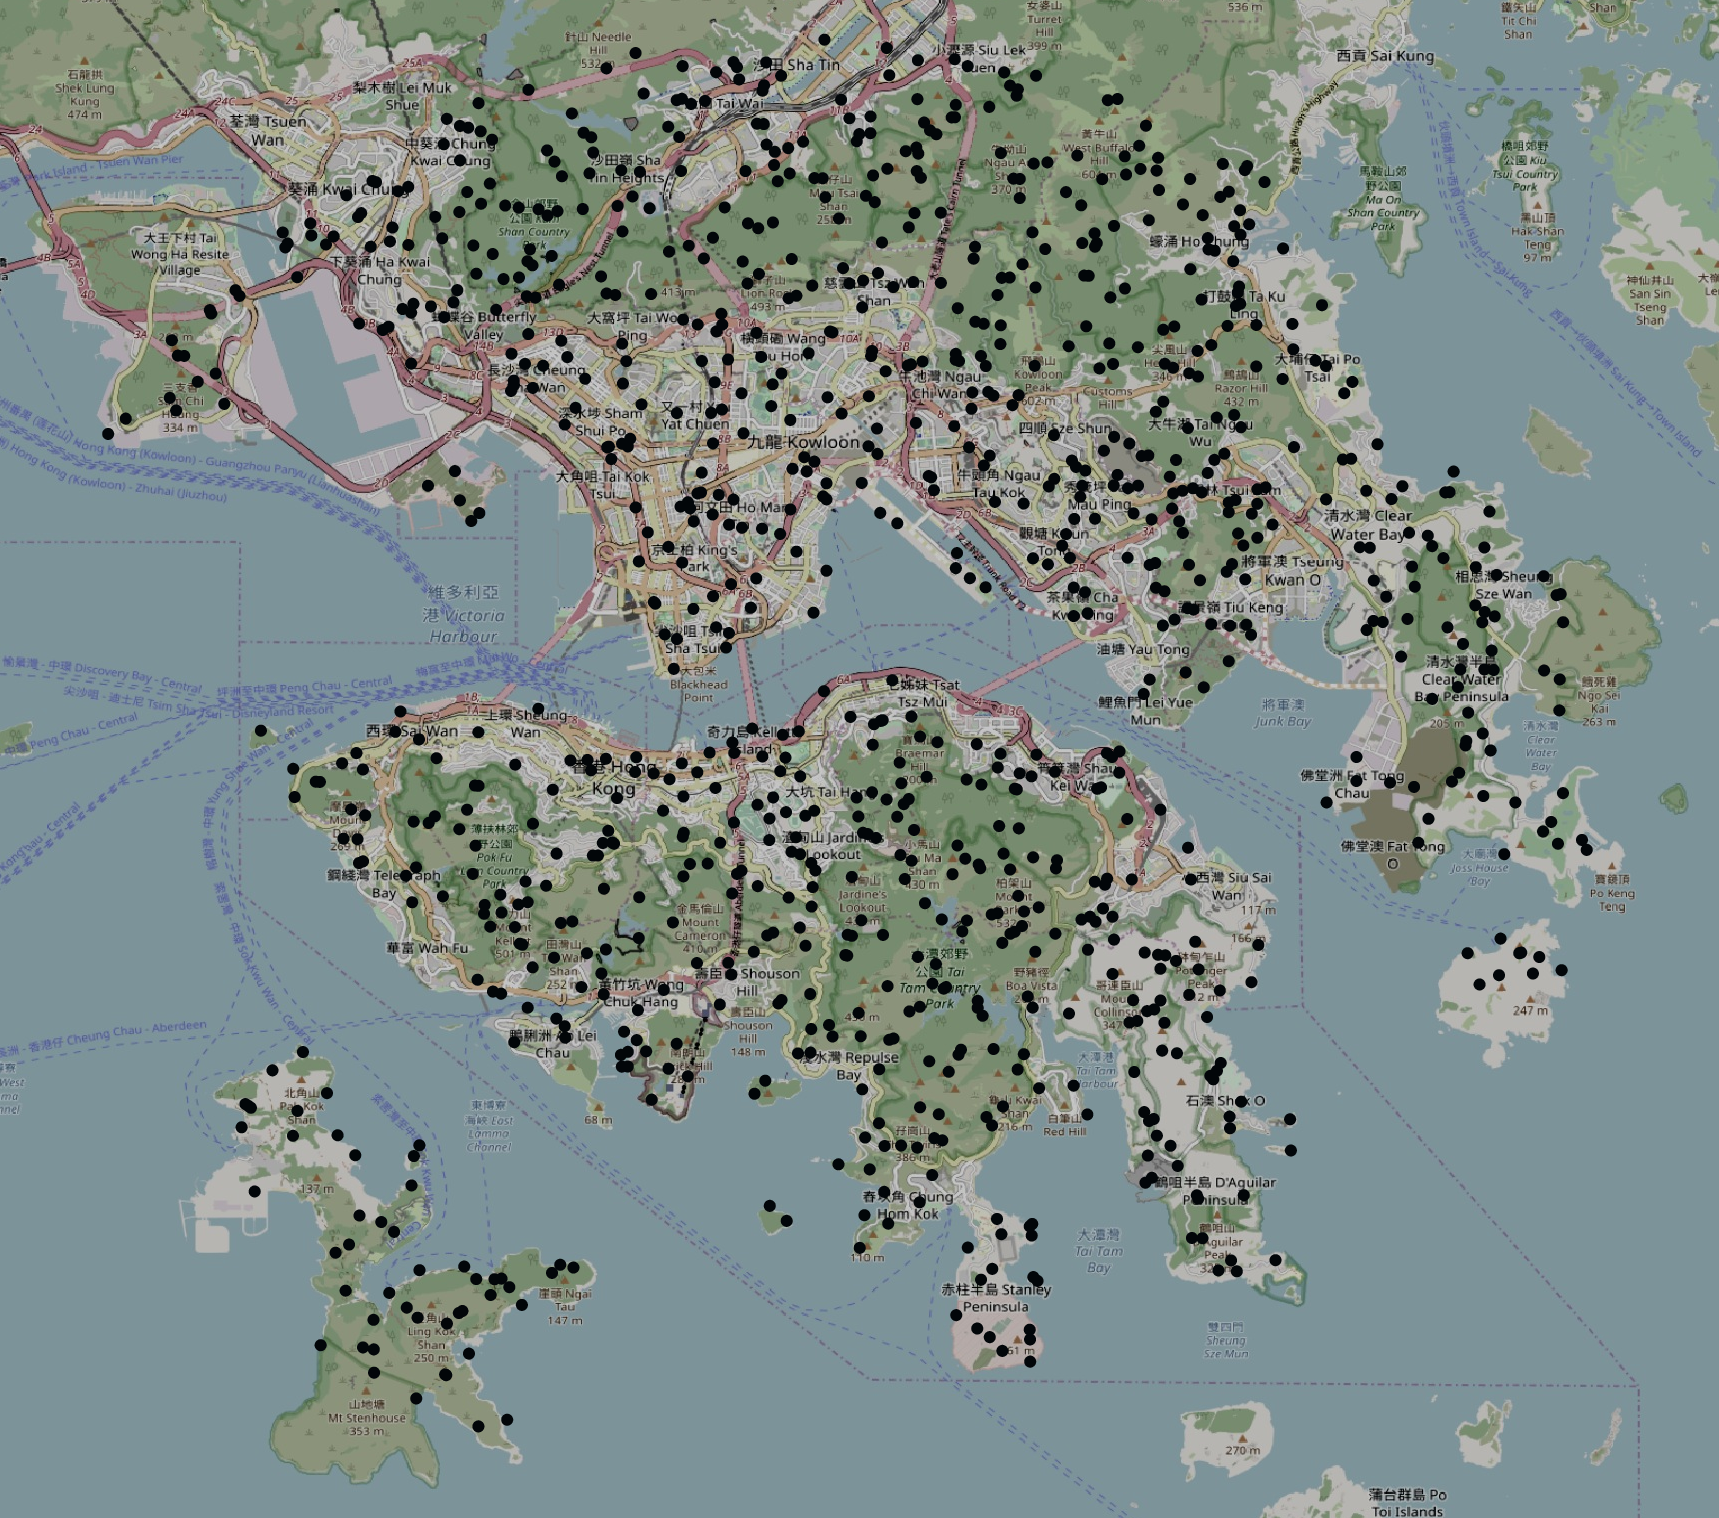
\includegraphics[trim={0 0 0 0},clip,scale=0.15]{HongKongSamples_.png}
\caption{\bf Sampling locations for map imagery (from Hong Kong).}
 \label{fig:parissample}
\end{figure} 



\subsection{Map imagery source.}\label{methodsimagery}

320$\times$320 pixel sized map images were sampled for 1692 cities using a zoom level of 16 (covering 750$\times$750m at the equator and down to 335$\times$335m at higher latitudes) using a custom style defined with the Google Static Maps API\cite{GoogleStatic2017} (see Figure~\ref{fig:maps} for examples of Paris, France). To ensure each map covers the same area, each image was cropped and resized before processing. The sampled city at the highest latitude was at 64 degrees north, so each image was cropped and resized to include a region of 335$\times$335m. 

The maps provide a high-level abstraction of road (black) and public transport (orange) networks, green space (green), and water bodies (blue). Any remaining space is coded white. Inconsistent map imagery from 25 South Korean cities (due to South Korean government restrictions on map data\cite{Badalge2018}) was removed from the dataset, reducing the number of cities to 1667. 1000 maps were sampled per city. The total dataset consists of nearly 1.7 million images.

\begin{figure}
\centering
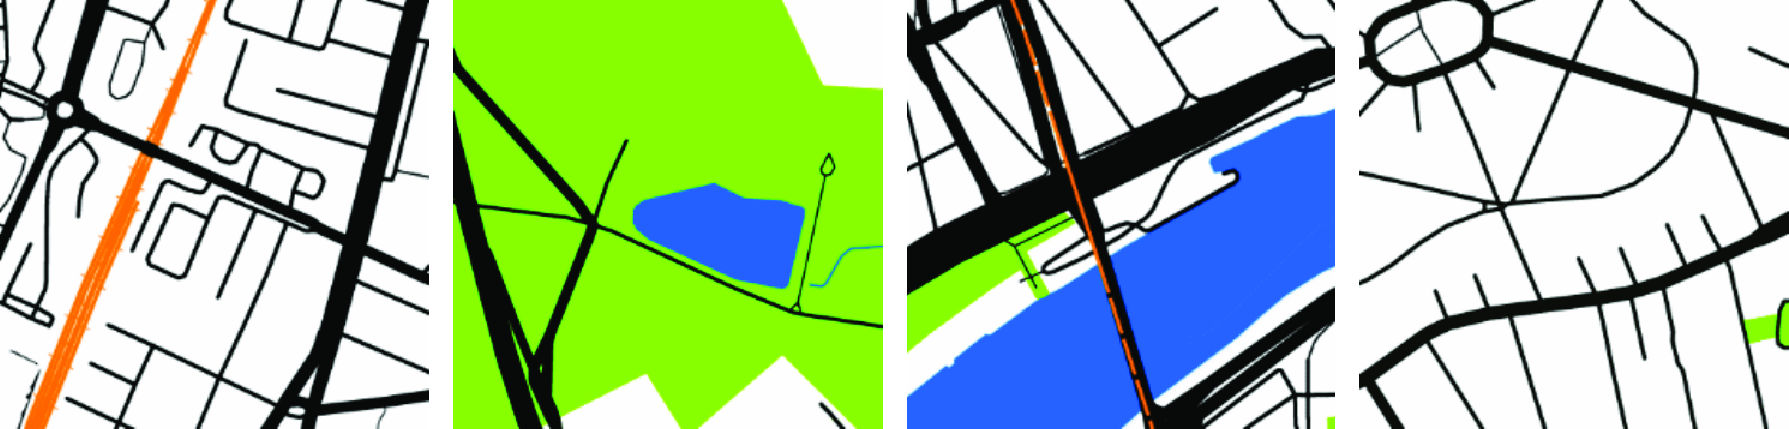
\includegraphics[trim={0 0 0 0},clip,scale=0.15]{BlockTypologies_Figures2-4.png}
\caption{\bf Four sample Google Maps training data images (from Paris, France)\cite{GoogleStatic2017}.}
 \label{fig:maps}
\end{figure} 

\subsection{Calculating block size, regularity, and colour counts.}\label{methodscalc}

Block size, regularity, and colour counts were calculated for each sampled image with Algorithm \ref{alg:floodfill}, using the Java 8 AWT toolkit\cite{Oracle2018}:

\begin{algorithm}[H]\label{alg:floodfill}
\SetAlgoLined
\KwResult{Histogram of region sizes and region regularity for a single image}
 Using latitude of image sample, crop the image to represent 335$\times$335 meters;\\
 Resize image back to 320$\times$320 pixels;\\
 Start at top left point of image;\\
 \While{White pixels are found}{
  Floodfill area using boundaries of all non-white colours (i.e. black, green, blue, orange);\\
  Count pixel size of region;\\
  Construct the smallest bounding box of the cloud of points in the region using the Fast Convex Hull algorithm\cite{Javagl2017,GoogleArchive2011};\\
  Use the difference of counted pixels between the bounding box size and the region size as measure of irregularity;\\
  Add size and regularity counts to corresponding (pre-specified) histogram bin;\\
  Locate next white pixel by iterating across rows and columns;\\
 }
 Count percentage of blue, orange, green, black, and white pixels in each image.\\
 Combine the two size and regularity histograms along with colour counts into a single histogram vector to be used in the SOM.\\
 \caption{Calculation of histograms of block sizes and regularity}
\end{algorithm}

Samples of size floodfills and regularity floodfills are shown in Figure \ref{fig:floodfilled}. Sample histograms used in the SOM are shown in Figure \ref{fig:mapsandHist}.

\begin{figure}
\centering
 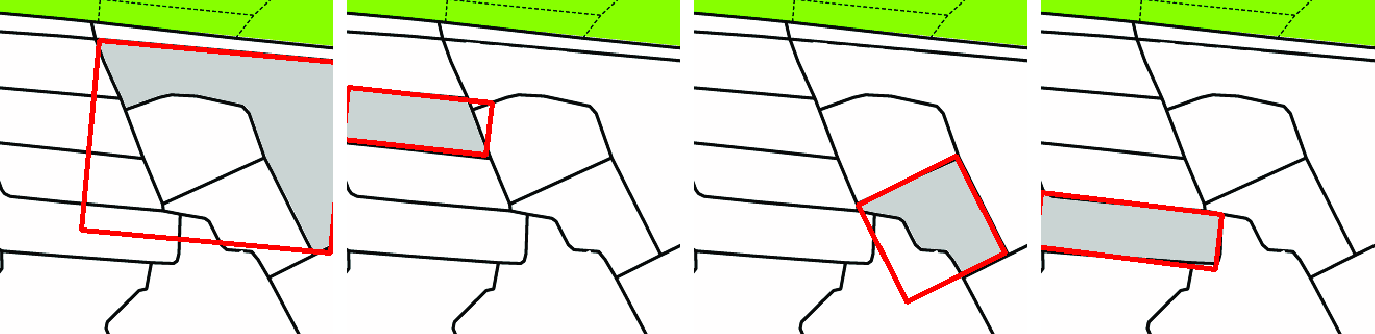
\includegraphics[trim={0 0 0 0},clip,scale=0.25]{BlockTypologies_Figures2-5.png}
\caption{\bf Results of flood filled city blocks showing flood fills of each individual region to determine region size (count of pixels in grey). Differences between region size and pixel counts within bounding boxes (outlined in red) are used as a measure of regularity.}
 \label{fig:floodfilled}
\end{figure} 

\subsection{City size and regularity histograms.}\label{methodshist}

Using the calculated counts, two vectors were constructed for each image, one each for block size and block regularity. The vectors were sorted into 15 histogram bins (the number of bins determined by Sturges' formula\cite{Sturges1926}, $\lceil \log_{2}n \rceil +1$, with $n$ being the number of data points). To reduce the clumping of data in the first bin, bins of increasing sizes were used to spread this data across all bins. The first bin starts with a size boundary of 1 and each following bin has a boundary of the current bin boundary times a multiplier. A multiplier of 2.3 was used to fit the maximum count size (320$\times$320 pixels = 102400) into the 15 bins.

The resulting histograms for sample map regions are shown in Figure \ref{fig:mapsandHist}. Histograms input into the SOM were constructed by combining the 15 bins of region size frequencies (on the left side) with the 15 bins of region regularity frequencies (second 15 bins) into a single histogram vector. In addition, the 5 colour pixel percentages are appended to the end of the histogram vector. Finally, the vector values are normalised into a range of 0 to 1.


\begin{figure}
\centering
 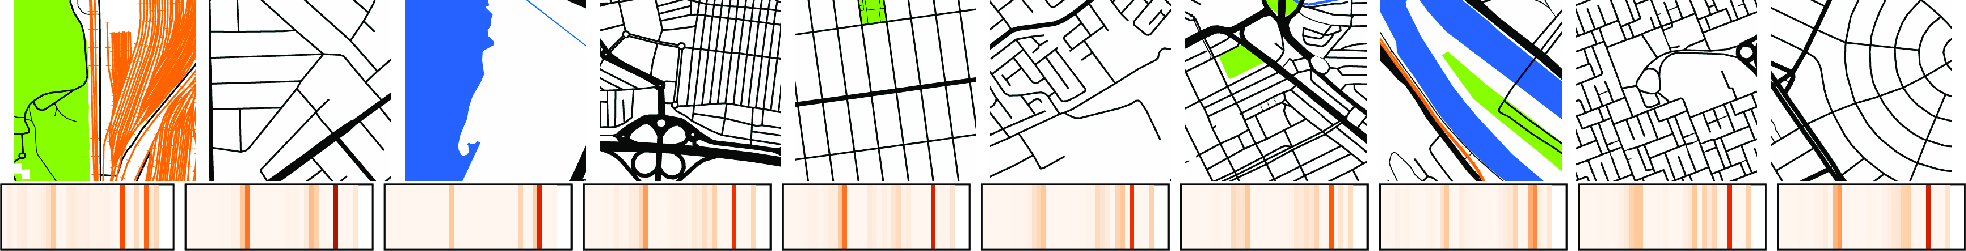
\includegraphics[trim={0 0 0 0},clip,scale=0.20]{BlockTypologies_Figures2-6.png}
\caption{\bf Samples of map regions (top) and resulting histograms (bottom). Region size, regularity, and colour counts are joined into a combined histogram vector, with size frequencies in the first 15 bins, regularity in the second 15 bins and colour pixel counts in the remaining 5 bins.}
 \label{fig:mapsandHist}
\end{figure} 

\subsection{Sorting map histograms in the self organising map.}\label{methodscluster}
The SOM methodology\cite{Kohonen1982} is a data driven technique that transforms a multi-dimensional data source into a lower dimensional space, commonly a two-dimensional map, while keeping the relative proximity of two datapoints intact. The distance in the lower dimensional representation is therefore a similarity index, calculated as the euclidean distance, of the higher dimensional space. Each point in the two-dimensional map has location (x,y) and is associated with a vector of values from the multi-dimensional space.

SOM is a generic, objective and robust methodology that has been deployed in many domains and is used for the visualisation of multi-dimensional data and data exploration\cite{Koleheimen2004}. This methodology was chosen for its ability to create two-dimensional maps of smoothly changing patterns from the original high-dimensional space. Additionally, the SOM map spans the extremes observed in the original data and allows for investigation on how the data is distributed, potential paths between two observations. 

The 1.7 million map histograms with 35 dimensions were the initial data space used to train the two-dimensional SOM. After the randomised initialisation of the 100x100 nodes of the SOM, a random selection of 5.4 million data points from the initial data space were used to transform the two-dimensional SOM to match it. This iterative process locates nodes that are similar to the training vector and morphs the values of the SOM nodes towards the training values. The number of iterations were determined by the minimum number of iterations to reach the greatest continuity among clusters. Training was stopped when the clusters started becoming discontinuous, checking every 150,000 iterations for a rapid increase in number of clusters. However, experimentally, we found that once a sufficient number of iterations were run, subsequent iterations only had small impacts on the results. 

This training is subjugated to a decay function for both magnitude (learning decay, $L_{i}$) and distance (radius decay, $D_{R}$) in the SOM. Radius decay was calculated using

\begin{equation} 
D_{R} = r_{0} e^{-\frac{i}{n} \log _{10} (r_{0})}
\end{equation}
where radius ($r_{0}$) is 50 (the width and height of the SOM was 100) and the current training iteration $i$ (of total iterations $n$ of 3.2 million). Learning decay is calculated as
\begin{equation} 
L_{i} = L_{0} e^{-\frac{i}{n}}
\end{equation}
where learn rate ($L_{0}$) = 0.05.

After the SOM was trained, each map histogram was classified to find the closest matching node in the SOM. The underlying imagery of the resulting trained SOM was visualised by tiling representative map images from each node (x,y) point in the SOM in Figure \ref{fig:somresults}. Areas with black have no associated map segments with that particular node's (x,y) location (about 5000 nodes). Most nodes are associated with multiple map segments that have similar characteristics. One notable outlier exists that accumulates more than 60,000 map segments of (0,99) with 385,967 maps that are all or nearly all white. Approximately 20 nodes contain 60,000 to 10,000 maps, about 200 contain 10,000 to 1000 maps, 5700 nodes contain 1000 to 1 map.

%0	99	385967
%99	8	58542
%46	99	50585


The node's (x,y) locations were encoded into RGB colour codes using a Java 8 port of Color2D\cite{Jackle2017,Steiger2015}. These colours were used in plotting the (x,y) typologies in QGIS\cite{QGIS2009}.


\subsection{KernelDensityEstimator2D.}\label{kerneldensity}

To create the city fingerprints, kernel density plots were made of the SOM x,y locations for each city using the KernelDensityEstimator2D (a bi-variate kernel density smoother for data) module from the Bayesian Evolutionary Analysis by Sampling Trees (BEAST) software package \cite{Suchard2018} with a smoothed grid size of 100.

% KernelDensityEstimator2D kde = new KernelDensityEstimator2D(dataXa, dataYa, null, 100, null); // 100 is smoothed grid size

\subsection{Aerosol Optical Depth (AOD) Dataset}\label{aod}
Two near-identical MODIS (Moderate Resolution Imaging Spectroradiometer) instruments are mounted upon the sun-synchronous polar-orbiting NASA satellites Terra and Aqua; these missions have over-pass times of approximately 10:30am and 1:30pm local time and were launched in 1999 and 2004, respectively. The MODIS resolution is 10 km $\times$ 10 km at nadir. The MOD04 and MYD04 L2 retrievals (V006) were downloaded and gridded to 0.05$^\circ$ x 0.05$^\circ$ (grid-spacing of approximately 5.6km). A range of different retrievable fields are available of which we used "Optical\_Depth\_Land\_And\_Ocean" (see Table B1 of Levy et al. (2013)\cite{Levy2013}), which represents a compromise between quality and coverage. These data were averaged to a monthly temporal resolution on this grid, and the number of MODIS pixels contributing to each averaged value were recorded. At each grid-point, a time-series decomposition into seasonal, trend and irregular (STL) components was applied\cite{Cleveland1990}. A slight modification to the code of the STL algorithm in the R stats package\cite{RCoreTeam2015} was made so that data were weighted by the number of observations involved in creating these observations. The trend component is estimated as a smooth function (via the locally weighted scatterplot smoothing, or LOESS, algorithm of Cleveland et al. (1992)\cite{Cleveland1992}), however the trend window parameter (defining the smoothing length scale for the trend term) was set sufficiently high that this term was effectively a linear term. From this, we derived the mean concentration at each grid-point accounting for long-term trend and seasonal fluctuations.

\subsection{NO$_{2}$ Dataset}\label{no2}
The tropospheric-column NO$_{2}$ data were derived from the TEMIS (Tropospheric Emission Monitoring Internet Service) OMI (Ozone Monitoring Instrument) tropospheric-column NO$_{2}$ (tcNO$_{2}$) database\cite{Boersma2007a}. Monthly gridded averages at 0.125$^\circ$ $\times$ 0.125$^\circ$ resolution (a grid-spacing of roughly 13km) were downloaded from the TEMIS website. These are based on the Level-2 tropospheric-column retrievals. While this provides little vertical information, the tcNO$_{2}$ product shows a good correlation with surface NO$_{2}$ concentrations, when averaged over a sufficient period. The OMI is mounted aboard NASA's sun-synchronous, polar-orbiting satellite Aura (launched July 2004). In normal operation, the OMI pixels are 13 km $\times$ 24 km at their finest (i.e. at nadir). The combination of the instruments wide swath (spanning about 2600 km) and the 14 orbits daily provides a global coverage every day, however retrievals are not possible everywhere, mainly due to clouds. Airborne aerosols and surface albedo are other significant sources of uncertainty. The monthly tcNO$_{2}$ data from 2005-2016 (complete years) were averaged at their native resolution.

\subsection{City fractions dataset}\label{gsvdata}
Middel et al. (2019,2018)\cite{Middel2019,Middel2018} derived fractional breakdowns from Google Street View (GSV) panorama images for 65 million locations across 75 cities of six urban form classes of sky, trees, buildings, impervious surfaces, pervious surfaces, and non-permanent objects (i.e. moving vehicles). Data for each location was indexed by city, latitude, and longitude. 

\subsection{Carbon intensity (FFDAS) dataset}\label{ffdasdata}
Rayner et al. (2010)\cite{Rayner2010a,Asefi-Najafabad2014} produced a high-resolution, global quantification of fossil fuel CO$_{2}$ emissions with their fossil fuel data assimilation system (FFDAS). We retrieved their gridded NetCDF yearly totals for 2010 (the latest year of this dataset) which provide values of $kgC/m^{2}/year$ at a 0.1$^\circ$ resolution. The quantified carbon sources include electricity generation and all other fossil fuel emissions (excluding shipping and aviation).

\subsection{SEDAC population density dataset}\label{populationdata}
The Gridded Population of the World, Version 4 (GPWv4) data collection\cite{CIESIN2018} from The Socioeconomic Data and Applications Center (SEDAC) was used to provide observations of population density. This provides global measures of population density at a resolution of 2.5 arc minutes (about 0.0416$^\circ$ or approximately 5km).

\subsection{Nearest neighbour averages}\label{knndata}
For each (x,y) point in the SOM, the groupings of (x,y) points required to include the 1000 nearest neighbours were calculated using the Euclidean Distance method from the Apache Commons Math library\cite{ApacheCommons2019}. Then for each point, these groupings were used to calculate mean values for each (x,y) point using the various observation datasets. (x,y) locations without associated map segments were assigned a value of NaN. The results were plotted on contour plots.

\subsection{City correlations}\label{correlations}
Mean averages for each city were generated using the same centroid area as in the "Map imagery sampling" section above, however locations were sampled at a 400$\times$400m resolution instead of the 1000 randomly selected locations. Using these locations, mean values of AOD and NO$_{2}$ were calculated for 1667 cities. A second set of city mean values were generated for 34 cities that matched the cities sampled for this study using the city fractions dataset.

Next, mean averages of pollution (AOD and NO$_{2}$) and of urban form fractions were calculated for each SOM(x,y) location. The latitude and longitude of each point (for the 1.7 million points) was used to look up an individual value from the gridded pollution datasets. For the city fractions dataset, latitude and longitude locations were matched to 0.0001 degree, for a total of approximately 8500 locations.

Finally, mean averages were calculated using the SOM(x,y) averages for the 1000 locations for 1667 and 34 cities for pollution and urban form respectively. Then the cor() function, using "pairwise.complete.obs" and "pearson", from the R stats package\cite{RCoreTeam2015} was used to find correlations between the two sets of computed city averages for the pollution and city fractions datasets.



%       row    column       cor     p
%aodAquaObs     xyAodAqua     0.5833058 0
%aodTerraObs     xyAodTerra     0.5678217 0
%no2Obs      xyNo2         0.5714648 0 
%        SVFByCity          SVFByXY  0.695137382 7.142315e-06
% imperviousByCity   imperviousByXY  0.858961761 8.040502e-119
%     movingByCity       movingByXY  0.973403215 0.000000e+00
%   perviousByCity     perviousByXY  0.432223290 1.068619e-02
%        skyByCity          skyByXY  0.754313707 2.576413e-07
%      treesByCity        treesByXY  0.330958635 5.588998e-02 

% AOD
%  AOD: Two near-identical MODIS (Moderate Resolution Imaging Spectroradiometer) instruments are mounted upon the sun-synchronous polar-orbiting NASA satellites Terra and Aqua; these missions have over-pass times of approximately 10:30am and 1:30pm local time and were launched in 1999 and 2004, respectively. The MODIS resolution is 10 km x 10 km at nadir. The MOD04 and MYD04 L2 retrievals (V006) were downloaded and gridded to 0.05° x 0.05° (grid-spacing of approximately 5.6km). A range of different retrievable fields are available of which we used "Optical_Depth_Land_And_Ocean" (see Table B1 of Levy et al., 2013), which represents a compromise between quality and coverage. These data were averaged to a monthly temporal resolution on this grid, and the number of MODIS pixels contributing to each averaged value were recorded. At each grid-point, a time-series decomposition into seasonal, trend and irregular (STL) components was applied (Cleveland et al., 1990). A slight modification to the code of the STL algorithm in the R stats package (R Core Team, 2015) was made so that data were weighted by the number of observations involved in creating these observations. The trend component is estimated as a smooth function (via the locally weighted scatterplot smoothing, or LOESS, algorithm of Cleveland et al., 1992), however the trend window parameter (defining the smoothing length scale for the trend term) was set sufficiently high that this term was effectively a linear term. From this, we derived the mean concentration at each grid-point accounting for long-term trend and seasonal fluctuations.

%NO2: The tropospheric-column NO2 data were derived from the TEMIS (Tropospheric Emission Monitoring Internet Service) OMI (Ozone Monitoring Instrument) tropospheric-column NO2 (tcNO2) database (Boersma et al., 2007). Monthly gridded averages at 0.125° x 0.125° resolution (a grid-spacing of roughly 13km) were downloaded from the TEMIS website. These are based on the Level-2 tropospheric-column retrievals. While this provides little vertical information, the tcNO2 product shows a good correlation with surface NO2 concentrations, when averaged over a sufficient period [REFS]. The OMI is mounted aboard NASA’s sun-synchronous, polar-orbiting satellite Aura (launched July 2004). In normal operation, the OMI pixels are 13 km x 24 km at their finest (i.e. at nadir). The combination of the instruments wide swath (spanning about 2600 km) and the 14 orbits daily provides a global coverage every day, however retrievals are not possible everywhere, mainly due to clouds. Airborne aerosols and surface albedo are other significant sources of uncertainty. The monthly tcNO2 data from 2005-2016 (complete years) were averaged at their native resolution.



% Estimates of Air Pollution: Air pollution for cities within the various global city clusters were derived from 3 global data sources namely, i) the, TEMIS OMI tropospheric-column NO2 database (Boersma et al., 2007), ii) the MODIS MOD04 and MYD04 L2 (AOD or aerosol data)(Chu et al., 2003) and iii) the Fossil Fuel Data Assimilation System (CO2 emissions estimates) (Rayner et al. 2010; Asefi-Najafabad et al 2014). Both the NO2 and AOD data were based on daily satellite overpasses of each city at 10.30am and 13.30pm local time, and recordings are obtained during cloud-free periods. By contrast, the CO2 emissions dataset is built upon high-resolution gridded population and night-light maps. These data were interpolated from global gridded data (at a resolution of 0.125°, 0.05°, and 0.1° latitude/longitude) to the locations of the 1667 clustered global cities. For each city, a difference was taken of the median of the sixteen surrounding points (N, NNE, NE, E, etc.) at twice the sampling radius of the city. Finally, CO2 emissions (in units of kgC/m2/y) were extracted from the latest available year (2010) of the Fossil Fuel Data Assimilation System dataset (Rayner et al. 2010; Asefi-Najafabad et al 2014). Further details on the processing of the satellite is described in Appendix A.


%the MODIS MOD04 and MYD04 L2 (AOD or aerosol data)(Chu et al., 2003). and AOD data was based on daily satellite overpasses of each city at 10.30am and 13.30pm local time, and recordings are obtained during cloud-free periods.

% AOD data from the NASA service LAADS-DAAC (Level-1 and Atmosphere Archive & %Distribution System, Distributed Active Archive Center, %https://ladsweb.modaps.eosdis.nasa.gov/).




